\documentclass{llncs}
\usepackage{times}
\usepackage[T1]{fontenc}

% Comentar para not MAC Users
%\usepackage[applemac]{inputenc}

\usepackage{a4}
%\usepackage[margin=3cm,nohead]{geometry}
\usepackage{epstopdf}
\usepackage{graphicx}
\usepackage{fancyvrb}
\usepackage{amsmath}
\usepackage[bookmarks=false]{hyperref}
%\renewcommand{\baselinestretch}{1.5}

\begin{document}
\mainmatter
\title{TP3: Camada de Ligação Lógica: Ethernet e Protocolo ARP}

\titlerunning{TP3: Camada de Ligação Lógica: Ethernet e Protocolo ARP}

\author{Diogo Afonso Costa \and Daniel Maia \and Vitor Castro}

\authorrunning{Diogo Afonso Costa \and Daniel Maia \and Vitor Castro}

\institute{
University of Minho, Department of  Informatics, 4710-057 Braga, Portugal\\
e-mail: \{a78034,a77531,a77870\}@alunos.uminho.pt
}

\date{}
\bibliographystyle{splncs}

\maketitle
\begin{abstract}
Resumo...
\end{abstract}

\section{Introdução}



\clearpage
\section{Parte I - Captura e análise de Tramas Ethernet}

\subsection{Exercício 1}
\subsubsection{Questão}\rule[-10pt]{0pt}{10pt}\\

Anote os endereços MAC de origem e de destino da trama capturada.

\subsubsection{Resposta}\rule[-10pt]{0pt}{10pt}\\

\textit{Destination}: Vmware\_d2:19:f0 (00:0c:29:d2:19:f0)
\textit{Source}: LcfcHefe\_66:65:4a (68:f7:28:66:65:4a)

\subsubsection{Realização}\rule[-10pt]{0pt}{10pt}\\

\begin{figure}
  \begin{center}
  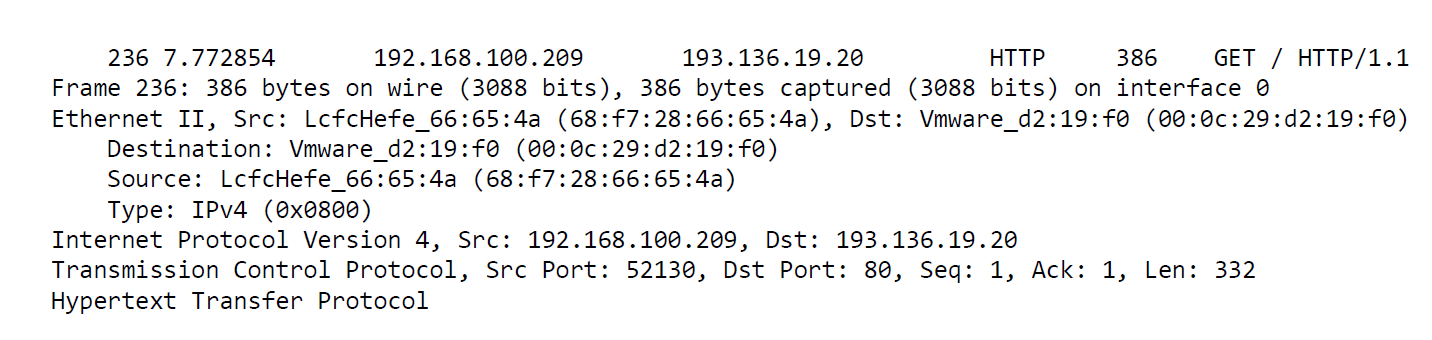
\includegraphics[scale=0.35]{imagens/MACAddrGET.png} 
  \end{center}
  \caption{Endereços MAC do HTTP GET.}
  \label{fig:mac_addr}
\end{figure} 

\clearpage
\subsection{Exercício 2}
\subsubsection{Questão}\rule[-10pt]{0pt}{10pt}\\

Identifique a que sistemas se referem. Justifique.

\subsubsection{Resposta}\rule[-10pt]{0pt}{10pt}\\

O MAC \textit{destination} refere ao comutador da rede local.
O MAC \textit{source} refere à máquina que enviou o pedido; neste caso, o computador utilizado.

\subsubsection{Realização}\rule[-10pt]{0pt}{10pt}\\

Ao nível da ligação de dados, as máquinas apenas comunicam com máquinas adjacentes.

\clearpage
\subsection{Exercício 3}
\subsubsection{Questão}\rule[-10pt]{0pt}{10pt}\\

Qual o valor hexadecimal do campo \textit{Type} da trama Ethernet? O que significa?

\subsubsection{Resposta}\rule[-10pt]{0pt}{10pt}\\

\textit{Type}: 0x0800; Este valor indica o tipo IPv4.

\subsubsection{Realização}\rule[-10pt]{0pt}{10pt}\\

\begin{figure}
  \begin{center}
  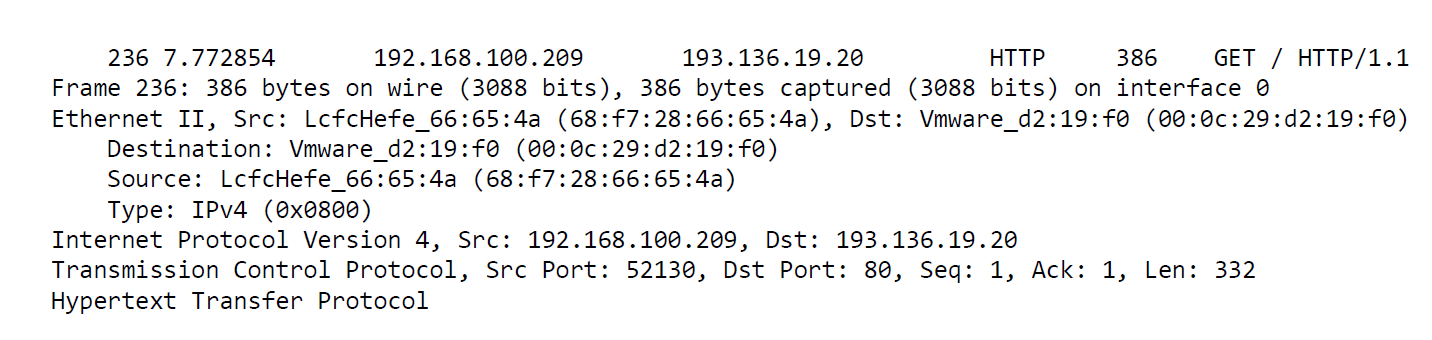
\includegraphics[scale=0.35]{imagens/MACAddrGET.png} 
  \end{center}
  \caption{O campo \textit{Type} da trama.}
  \label{fig:frame_field}
\end{figure} 

\clearpage
\subsection{Exercício 4}
\subsubsection{Questão}\rule[-10pt]{0pt}{10pt}\\

Quantos bytes são usados desde o início da trama até ao caractere ASCII “G” do método HTTP GET? Calcule e indique, em percentagem, a sobrecarga (overhead) introduzida pela pilha protocolar no envio do HTTP GET.

\subsubsection{Resposta}\rule[-10pt]{0pt}{10pt}\\

Até ao caractere "G", existem 54 bytes dos 386 bytes do método, resultando num overhead percentual de (54/386) * 100 = 14\%

\subsubsection{Realização}\rule[-10pt]{0pt}{10pt}\\

\begin{figure}
  \begin{center}
  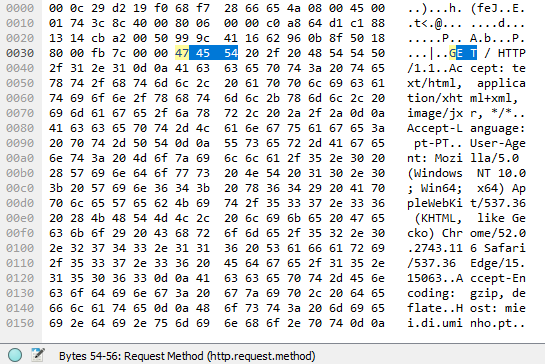
\includegraphics[scale=0.35]{imagens/HTTPbytes.png} 
  \end{center}
  \caption{O byte com o caratere "G" aparece após 54 outros.}
  \label{fig:http_bytes}
\end{figure} 

\clearpage
\subsection{Exercício 5}
\subsubsection{Questão}\rule[-10pt]{0pt}{10pt}\\

Em ligações com fios pouco susceptíveis a erros, nem sempre as NICs geram o código de detecção de erros. Através de visualização direta de uma trama capturada, verifique se o campo FCS está visível, i.e., se está a ser utilizado. Aceda à opção Edit/Preferences/Protocols/Ethernet e indique que é assumido o uso do campo FCS. Verifique qual o valor hexadecimal desse campo na trama
capturada. Que conclui? Reponha a configuração original.

\subsubsection{Resposta}\rule[-10pt]{0pt}{10pt}\\

O valor hexadecimal FCS da trama é 0x0d0a0d0a, mas deveria ser 0x971613cf. Disto conclui que a NIC não gerou código de verificação de erros, visto que, se a trama estivesse incorreta, o pacote teria sido enviado.

\subsubsection{Realização}\rule[-10pt]{0pt}{10pt}\\

\begin{figure}
  \begin{center}
  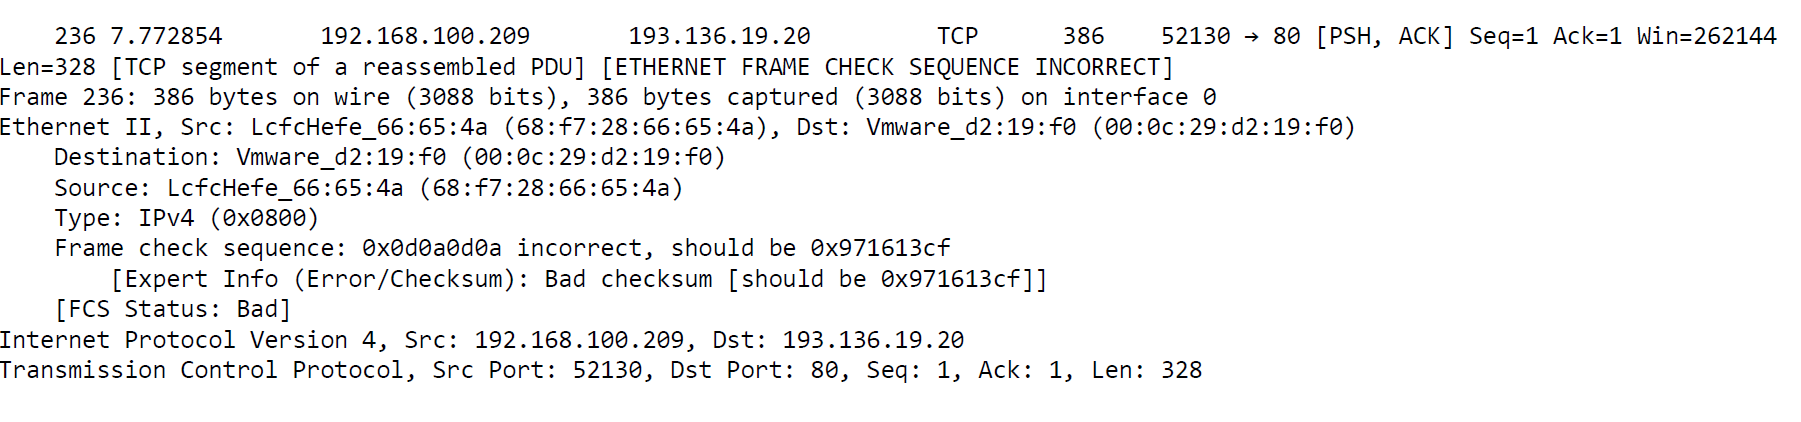
\includegraphics[scale=0.35]{imagens/FCS.png} 
  \end{center}
  \caption{Se o pacote tivesse um erro, não seria enviado e, por extensão, capturado.}
  \label{fig:fcs_field}
\end{figure} 

\clearpage
\subsection{Exercício 6}
\subsubsection{Questão}\rule[-10pt]{0pt}{10pt}\\

Qual é o endereço Ethernet da fonte? A que sistema de rede corresponde? Justifique.

\subsubsection{Resposta}\rule[-10pt]{0pt}{10pt}\\

\textit{Address}: Vmware_d2:19:f0 (00:0c:29:d2:19:f0)
Este endereço corresponde ao comutador da rede local visto que, ao nível dos dados, máquinas apenas comunicam com as máquinas adjacentes através do protocolo ARP.

\subsubsection{Realização}\rule[-10pt]{0pt}{10pt}\\

\begin{figure}
  \begin{center}
  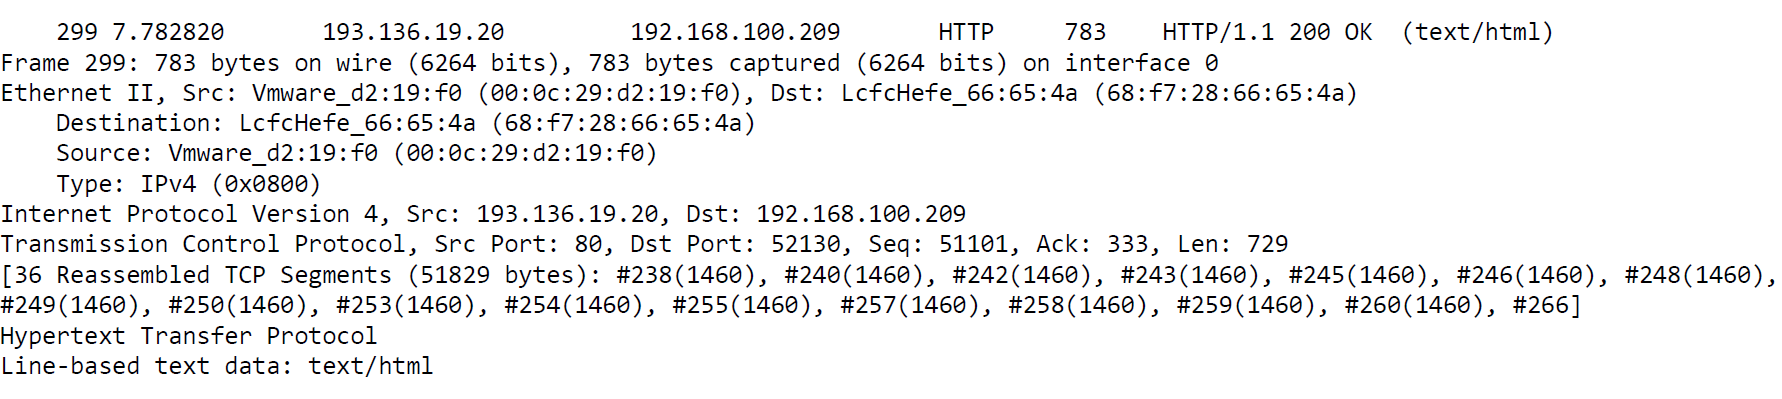
\includegraphics[scale=0.35]{imagens/HTTPresponse.png} 
  \end{center}
  \caption{O endereço Ethernet da fonte da resposta.}
  \label{fig:ethernet_response_source}
\end{figure}

\clearpage
\subsection{Exercício 7}
\subsubsection{Questão}\rule[-10pt]{0pt}{10pt}\\

Qual é o endereço MAC do destino? A que sistema corresponde?

\subsubsection{Resposta}\rule[-10pt]{0pt}{10pt}\\

\textit{Address}: LcfcHefe_66:65:4a (68:f7:28:66:65:4a)
Este endereço corresponde ao computador utilizado, que originalmente enviou o pedido HTTP GET.

\subsubsection{Realização}\rule[-10pt]{0pt}{10pt}\\

\begin{figure}
  \begin{center}
  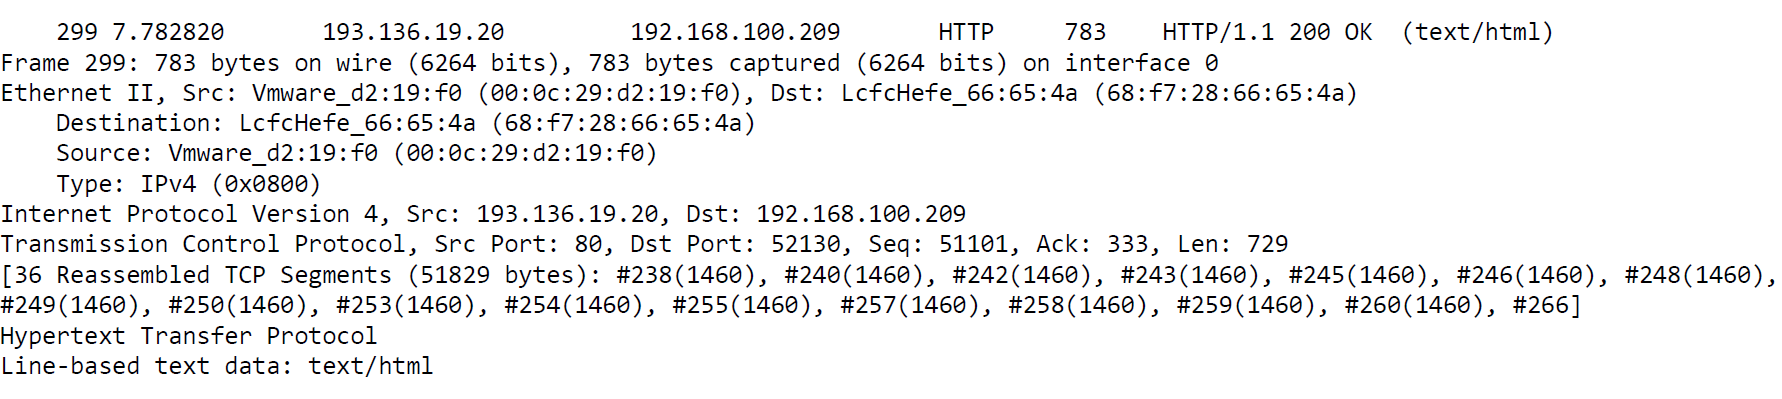
\includegraphics[scale=0.35]{imagens/HTTPresponse.png} 
  \end{center}
  \caption{O endereço Ethernet do destino da resposta.}
  \label{fig:ethernet_response_dest}
\end{figure}

\clearpage
\subsection{Exercício 8}
\subsubsection{Questão}\rule[-10pt]{0pt}{10pt}\\

Atendendo ao conceito de desencapsulamento protocolar, identifique os vários protocolos contidos na trama recebida.

\subsubsection{Resposta}\rule[-10pt]{0pt}{10pt}\\

Na trama capturada está contido um protocolo Ethernet II, no qual está encapsulado um protocolo IPv4 que, por sua vez, transporta um protocolo TCP, no qual está contido um protocolo Hypertext Transfer Protocol (HTTP).

\subsubsection{Realização}\rule[-10pt]{0pt}{10pt}\\

\begin{figure}
  \begin{center}
  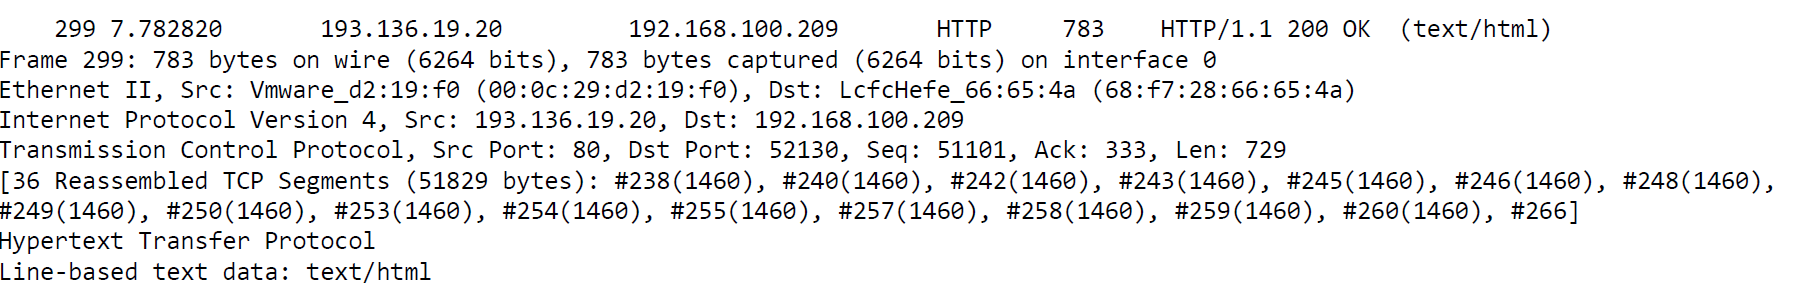
\includegraphics[scale=0.35]{imagens/fields.png} 
  \end{center}
  \caption{Os protocolos contidos na trama de resposta.}
  \label{fig:response_fields}
\end{figure}


% 4. Protocolo ARP ---------
\clearpage
\subsection{Exercício 9}
\subsubsection{Questão}\rule[-10pt]{0pt}{10pt}\\

Observe o conteúdo da tabela ARP. Diga o que significa cada uma das colunas?

\subsubsection{Resposta}\rule[-10pt]{0pt}{10pt}\\

A versão linux instalada na máquina na qual este exercício foi realizado não tem o pacote \textit{ARP} disponível pois este foi deprecado. Contudo, o comando \texttt{ip neigh}, realiza a mesma operação, isto é, permite observar o conteúdo da tabela \textit{ARP}.

Desta forma, consultando o manuel referente ao comando a cima mencionado (\texttt{man ip-neighbour}), percebe-se que o \textit{output} é segmentado em 4 colunas. A primeira indica o endereço IP da interface da máquina na vizinhança, à qual se refere a entrada na tabela. A segunda coluna, traduz a interface na qual o \textit{host} da vizinhança se encontra ligado. A terceira coluna apresenta o endereço MAC do \textit{host} a que esta entrada na tabela se refere. Por último, a quarta coluna indica o estado da ligação entre os dois sistemas.

\subsubsection{Realização}\rule[-10pt]{0pt}{10pt}\\

\begin{figure}
  \begin{center}
	  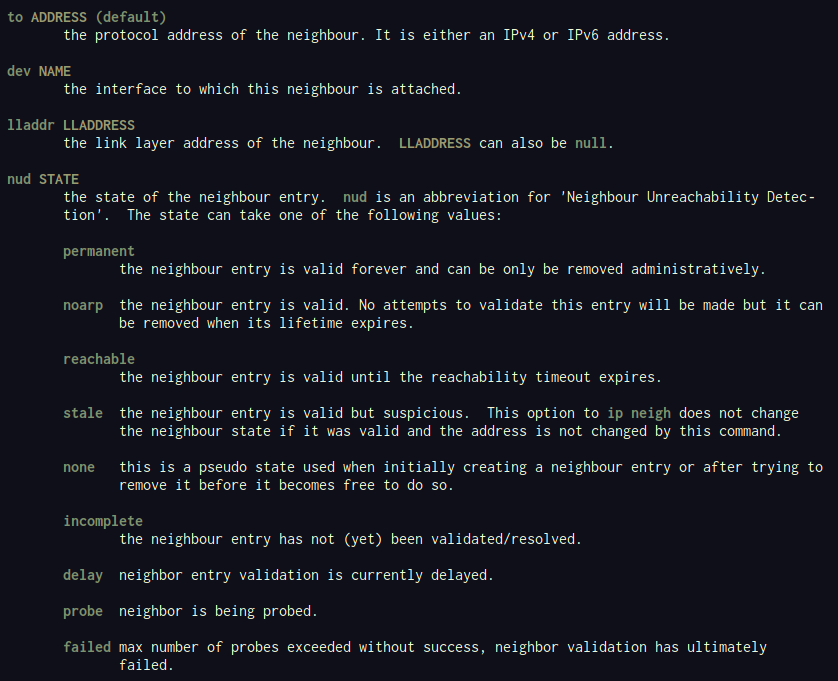
\includegraphics[scale=0.5]{./imagens/ip_neigh.png} 
  \end{center}
	\caption{Manual do comando \texttt{ip neigh}.}
  \label{fig:ip_neigh}
\end{figure} 


\clearpage
\subsection{Exercício 10}
\subsubsection{Questão}\rule[-10pt]{0pt}{10pt}\\

Qual é o valor hexadecimal dos endereços origem e destino na trama Ethernet que contém a mensagem com o pedido ARP (ARP Request)? Como interpreta e justifica o endereço destino usado?

\subsubsection{Resposta}\rule[-10pt]{0pt}{10pt}\\

Endereço origem: 2c:60:0c:6b:85:44

Endereço destino: ff:ff:ff:ff:ff:ff (broadcast)

A estratégia utilizada para resolver o exercício foi fazendo \textit{ping} para outra máquina do laboratório, nomeadamente, 192.168.100.205.

Desta forma, a máquina que estava a relizar o \textit{ping} apenas tinha a informação do IP da interface da máquina destino. No entanto, dado que o \textit{host} destino se encontra na vizinhança da máquina de origem, é possível enviar a trama sem que esta vá ao AP. Para tal é usado o protocolo ARP por forma a descobrir o MAC do \textit{host} para que a comunicação seja feita diretamente.

Deste modo, é enviado para todos os sistemas que se encontram na mesma rede local um ARP \textit{request}, por forma a descobrir o endereço MAC a que pertence o IP 192.168.100.205, daí o endereço de destino ser ff:ff:ff:ff:ff:ff. 

\subsubsection{Realização}\rule[-10pt]{0pt}{10pt}\\

\begin{figure}
  \begin{center}
	  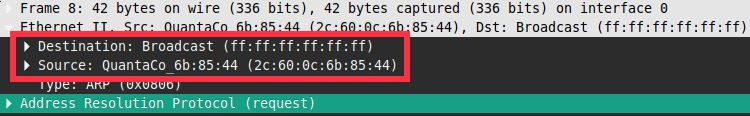
\includegraphics[scale=0.6]{./imagens/arp_request.png} 
  \end{center}
	\caption{Pedido \textit{ARP} enviado em \textit{broadcast}.}
  \label{fig:arp_request}
\end{figure} 


\clearpage
\subsection{Exercício 11}
\subsubsection{Questão}\rule[-10pt]{0pt}{10pt}\\

Qual o valor hexadecimal do campo tipo da trama Ethernet? O que indica?

\subsubsection{Resposta}\rule[-10pt]{0pt}{10pt}\\

\texttt{Type: ARP (0x0806)} 

Significa que a trama \textit{Ethernet} leva encapsulado o protocolo ARP.

\subsubsection{Realização}\rule[-10pt]{0pt}{10pt}\\

\begin{figure}
  \begin{center}
	  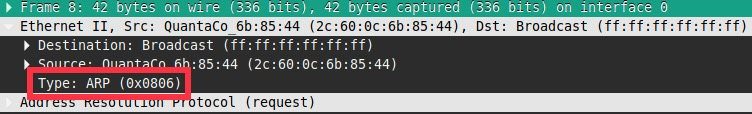
\includegraphics[scale=0.6]{./imagens/arp_request_type.png} 
  \end{center}
	\caption{Tipo da trama \textit{Ethernet}.}
  \label{fig:arp_request_type}
\end{figure} 


\clearpage
\subsection{Exercício 12}
\subsubsection{Questão}\rule[-10pt]{0pt}{10pt}\\

Qual o valor do campo ARP opcode? O que especifica?

\subsubsection{Resposta}\rule[-10pt]{0pt}{10pt}\\

\texttt{Opcode: request (1)}

Segundo o padrão descrito no RFC826 \cite{RFC0826}:
	\emph{"The opcode is to determine if this is a request (which may cause a reply) or a reply to a previous request.  16 bits for this is overkill, but a flag (field) is needed."}

Desta forma, pode-se afirmar que a trama em questão representa um ARP \textit{request}.

\subsubsection{Realização}\rule[-10pt]{0pt}{10pt}\\

\begin{figure}
  \begin{center}
	  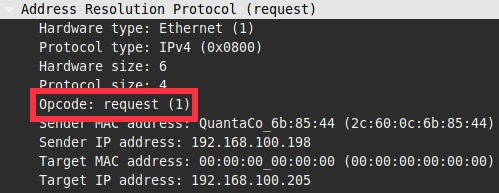
\includegraphics[scale=0.6]{./imagens/arp_request_opcode.png} 
  \end{center}
	\caption{Valor do \textit{opcode} do ARP \textit{request}.}
  \label{fig:arp_request_opcode}
\end{figure} 


\clearpage
\subsection{Exercício 13}
\subsubsection{Questão}\rule[-10pt]{0pt}{10pt}\\

Identifique que tipo de endereços estão contidos na mensagem ARP? Que conclui?

\subsubsection{Resposta}\rule[-10pt]{0pt}{10pt}\\

Os endereços contidos na mensagem ARP são os seguintes:

\begin{itemize}
	\item Sender MAC address: 2c:60:0c:6b:85:44

	\item Sender IP address: 192.168.100.198

	\item Target MAC address: 00:00:00:00:00:00 

	\item Target IP address: 192.168.100.254
\end{itemize}

Efetivamente, o facto de o \textit{Target MAC address} estar todo a zero significa que está à espera de ser preenchido, assim que o \textit{Target IP address} faça correspondência na máquina de destino.

\subsubsection{Realização}\rule[-10pt]{0pt}{10pt}\\

\begin{figure}
  \begin{center}
	  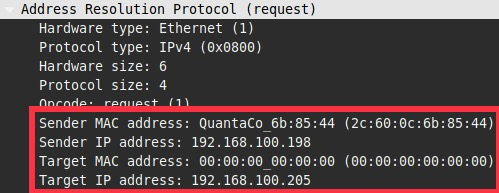
\includegraphics[scale=0.6]{./imagens/arp_request_addr.png} 
  \end{center}
	\caption{Endereços contidos na mensagem ARP.}
  \label{fig:arp_request_addr}
\end{figure} 


\clearpage
\subsection{Exercício 14}
\subsubsection{Questão}\rule[-10pt]{0pt}{10pt}\\

Explicite que tipo de pedido ou pergunta é feita pelo host de origem?

\subsubsection{Resposta}\rule[-10pt]{0pt}{10pt}\\

O \textit{host} de origem quer saber qual o endereço MAC da máquina que tem como IP da interface 192.168.100.205.


\clearpage
\subsection{Exercício 15.a)}
\subsubsection{Questão}\rule[-10pt]{0pt}{10pt}\\

Qual o valor do campo ARP opcode? O que especifica?

\subsubsection{Resposta}\rule[-10pt]{0pt}{10pt}\\

\texttt{Opcode: reply (2)}

Este valor significa que esta trama é a resposta a uma trama ARP \textit{request} recebida anteriormente.

\subsubsection{Realização}\rule[-10pt]{0pt}{10pt}\\

\begin{figure}
  \begin{center}
	  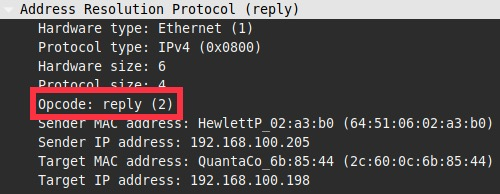
\includegraphics[scale=0.6]{./imagens/arp_reply_opcode.png} 
  \end{center}
	\caption{Campo \textit{opcode} do ARP \textit{reply}.}
  \label{fig:arp_reply_opcode}
\end{figure} 


\clearpage
\subsection{Exercício 15.b)}
\subsubsection{Questão}\rule[-10pt]{0pt}{10pt}\\

Em que posição da mensagem ARP está a resposta ao pedido ARP ?

\subsubsection{Resposta}\rule[-10pt]{0pt}{10pt}\\

\begin{itemize}
	\item Sender MAC address: 64:51:06:02:a3:b0
\end{itemize}

\subsubsection{Realização}\rule[-10pt]{0pt}{10pt}\\

\begin{figure}
  \begin{center}
	  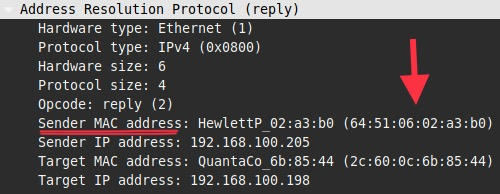
\includegraphics[scale=0.6]{./imagens/arp_reply_resp.png} 
  \end{center}
	\caption{Campo com a resposta ao pedido ARP.}
  \label{fig:arp_reply_resp}
\end{figure} 


\clearpage
\subsection{Exercício 16}
\subsubsection{Questão}\rule[-10pt]{0pt}{10pt}\\

Com auxílio do comando ifconfig obtenha os endereços Ethernet das interfaces dos diversos routers.

\subsubsection{Resposta}\rule[-10pt]{0pt}{10pt}\\

\begin{itemize}
  \item MAC Router n1 (eth0): 00:00:00:aa:00:00
  \item MAC Router n2 (eth0): 00:00:00:aa:00:01
  \item MAC Router n2 (eth1): 00:00:00:aa:00:02
  \item MAC Router n3 (eth0): 00:00:00:aa:00:03
\end{itemize}

Pode-se observar que as interfaces ligadas são a eth0 (de n1) e eth0 (de n2), relativas ao caminho entre \textbf{n1} e \textbf{n2}, tal como eth1 (de n2) e eth0 (de n3), correspondentes ao caminho entre \textbf{n2} e \textbf{n3}.

\subsubsection{Realização}\rule[-10pt]{0pt}{10pt}\\

\begin{figure}
  \begin{center}
    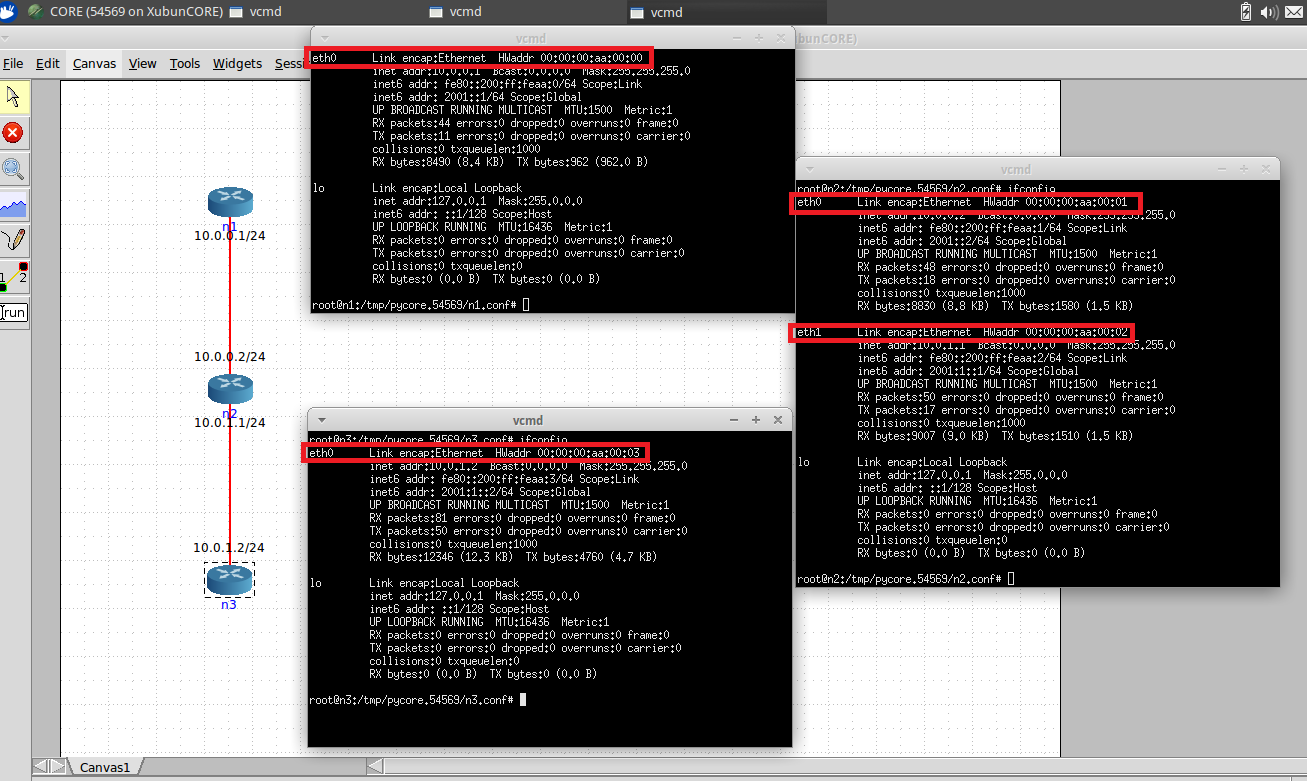
\includegraphics[scale=0.6]{./imagens/ifconfig.png} 
  \end{center}
  \caption{Endereços de interfaces.}
  \label{fig:arp_reply_resp}
\end{figure} 

\clearpage
\subsection{Exercício 17}
\subsubsection{Questão}\rule[-10pt]{0pt}{10pt}\\

Usando o comando arp obtenha as caches arp dos diversos sistemas.

\subsubsection{Resposta}\rule[-10pt]{0pt}{10pt}\\

As caches ARP inicialmente estão vazias, como seria de esperar, pois ainda não houve qualquer tipo de comunicação.

\subsubsection{Realização}\rule[-10pt]{0pt}{10pt}\\

\begin{figure}
  \begin{center}
    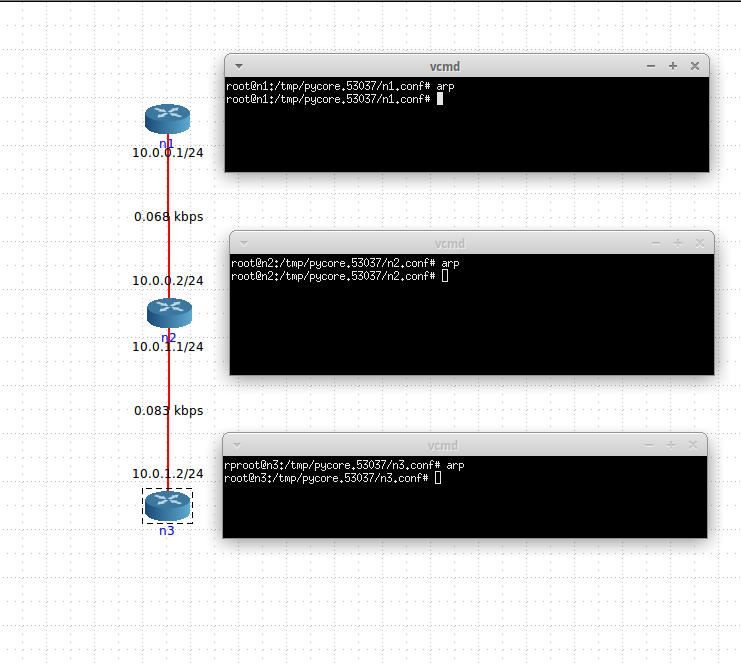
\includegraphics[scale=0.6]{./imagens/5.17.png} 
  \end{center}
  \caption{Caches ARP vazias.}
  \label{fig:arp_reply_resp}
\end{figure} 

\clearpage
\subsection{Exercício 18}
\subsubsection{Questão}\rule[-10pt]{0pt}{10pt}\\

Faça ping de n1 para n2. Que modificações observa nas caches ARP desses sistemas? Faça ping de n1 para n3. Consulte as caches ARP. Que conclui?

\subsubsection{Resposta}\rule[-10pt]{0pt}{10pt}\\

Depois de feito o ping de \textbf{n1} para \textbf{n2}, a tabela ARP de \textbf{n1} passou a conhecer o MAC address relativo à interface eth0 do router \textbf{n2}. Do mesmo modo, o router \textbf{n2} passou a conhecer o router \textbf{n1} na interface eth0.

Depois de fazer ping de \textbf{n1} para \textbf{n3}, a tabela ARP de \textbf{n1} manteve-se, uma vez que o protocolo ARP só permite conhecer as máquinas adjacentes. No entanto, o router \textbf{n2}, como foi utilizado para encaminhamento, passou a conhecer a interface eth0 do router \textbf{n3} que, por sua vez passou a conhecer a interface eth1 do router \textbf{n2}.

\subsubsection{Realização}\rule[-10pt]{0pt}{10pt}\\

\begin{figure}
  \begin{center}
    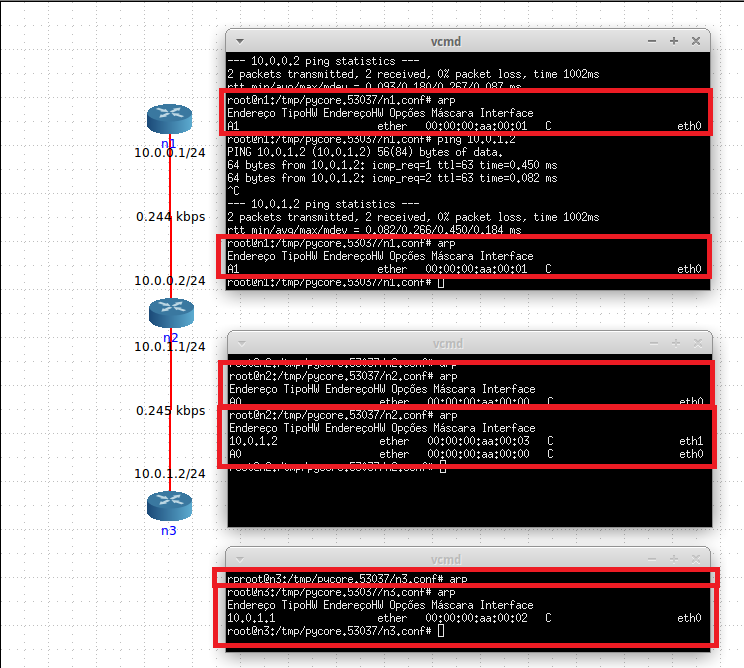
\includegraphics[scale=0.6]{./imagens/5.18.png} 
  \end{center}
  \caption{Atualização de caches ARP.}
  \label{fig:arp_reply_resp}
\end{figure} 

\clearpage
\subsection{Exercício 19}
\subsubsection{Questão}\rule[-10pt]{0pt}{10pt}\\

Em n1 remova a entrada correspondente a n2. Coloque uma nova entrada para n2 com endereço Ethernet inexistente. O que acontece?

\subsubsection{Resposta}\rule[-10pt]{0pt}{10pt}\\

\textbf{n1} conhecia, pelo ARP, o endereço IP da interface do router \textbf{n2}. Quando, na tabela ARP, removemos a entrada conhecida e adicionamos outra, com o mesmo IP mas com um endereço Ethernet inexistente, os pacotes são enviados para o endereço inexistente (no caso, utilizou-se 00:00:00:aa:00:04). Este envio é errado pois aquele endereço não existe, havendo perda total de pacotes. Este erro não é corrigido pois é suposto a tabela ARP estar correta.

\subsubsection{Realização}\rule[-10pt]{0pt}{10pt}\\

\begin{figure}
  \begin{center}
    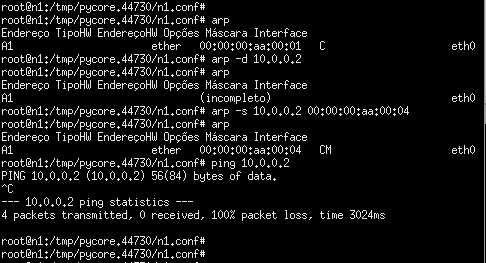
\includegraphics[scale=0.6]{./imagens/5.19.png} 
  \end{center}
  \caption{Tabela ARP com entradas erradas.}
  \label{fig:arp_reply_resp}
\end{figure} 

\clearpage
\subsection{Exercício 20}
\subsubsection{Questão}\rule[-10pt]{0pt}{10pt}\\

Faça ping de n6 para n5. Sem consultar a tabela ARP anote a entrada que, em sua opinião, é criada na tabela ARP de n6. Verifique, justificando, se a sua interpretação sobre a operação da rede Ethernet e protocolo ARP estava correto.

\subsubsection{Resposta}\rule[-10pt]{0pt}{10pt}\\

Como esperado, a tabela ARP de \textbf{n6} passou a conter o endereço Ethernet e IP do host 5. Como fazem parte da mesma sub-rede \textbf{10.0.2.x/24} e estão diretamente ligados, seria expectável que isto acontecesse. De facto, o \textit{switch} não tem qualquer impacto nas tabelas ARP, uma vez que funciona apenas como redirecionador de pacotes, não tendo interferência àquele nível de rede.

\subsubsection{Realização}\rule[-10pt]{0pt}{10pt}\\

\begin{figure}
  \begin{center}
    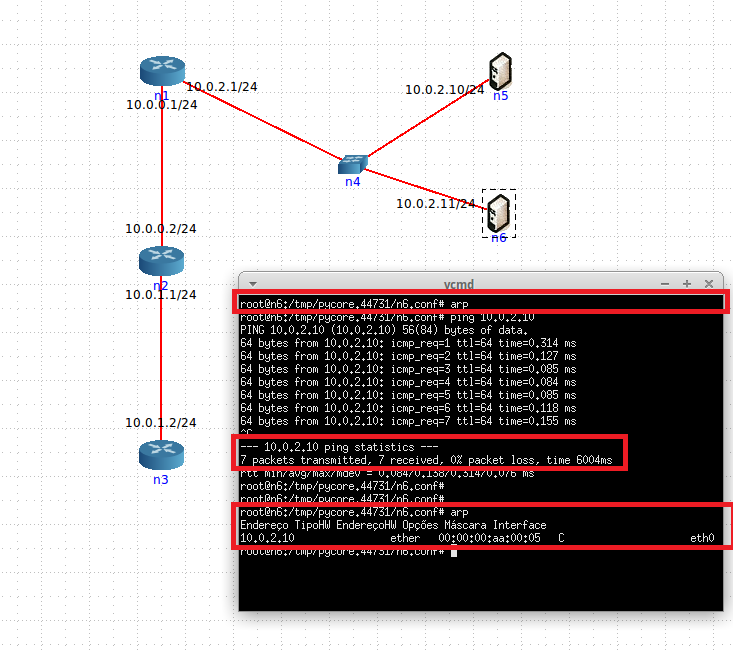
\includegraphics[scale=0.6]{./imagens/5.20.png} 
  \end{center}
  \caption{Tabela ARP atualizada com endereço de host.}
  \label{fig:arp_reply_resp}
\end{figure} 

\clearpage
\section{Parte II - ARP Gratuito}

\subsection{Exercício 1}
\subsubsection{Questão}\rule[-10pt]{0pt}{10pt}\\

Identifique um pacote de pedido ARP gratuito originado pelo seu sistema. Verifique quantos pacotes ARP gratuito foram enviados e com que intervalo temporal?

\subsubsection{Resposta}\rule[-10pt]{0pt}{10pt}\\

Analisando a captura de dados do Wireshark, verificou-se o envio de dois pacotes de ARP Gratuito em t = 15.631251s e t = 408.067672s (~ 392s). Com o intuito de confirmar o resultado, repetiu-se a experiência, capturando de novo dois pacotes de ARP Gratuito, que, desta vez foram enviados em t = 13.988762s e t = 641.373163s (~ 627s).

\subsubsection{Realização}\rule[-10pt]{0pt}{10pt}\\

\begin{figure}[h]
  \centering
  \begin{subfigure}{.4\textwidth}
    \centering
    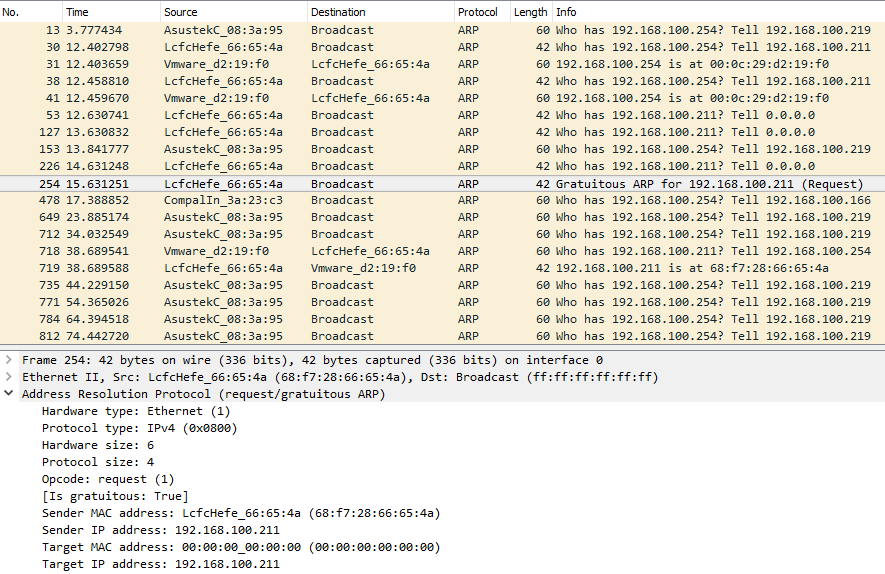
\includegraphics[width=0.98\linewidth]{./imagens/ARPG1_1.png}
  \end{subfigure}%
  \begin{subfigure}{.4\textwidth}
    \centering
    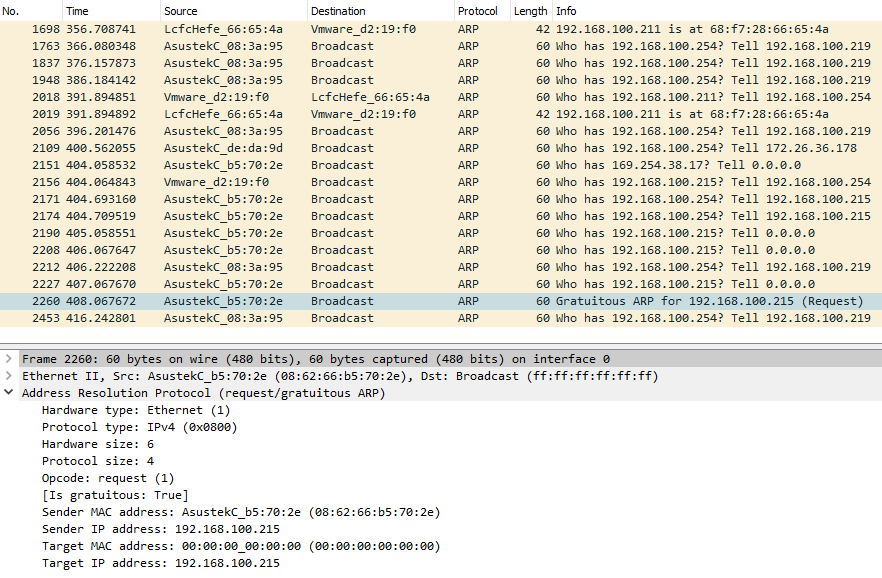
\includegraphics[width=0.98\linewidth]{./imagens/ARPG1_2.png}
  \end{subfigure}%
  \caption{2 pacotes de ARP Gratuito capturados com um intervalo de 392s.}
  \label{fig:arpg_1}
\end{figure}

\begin{figure}[h]
  \centering
  \begin{subfigure}{.4\textwidth}
    \centering
    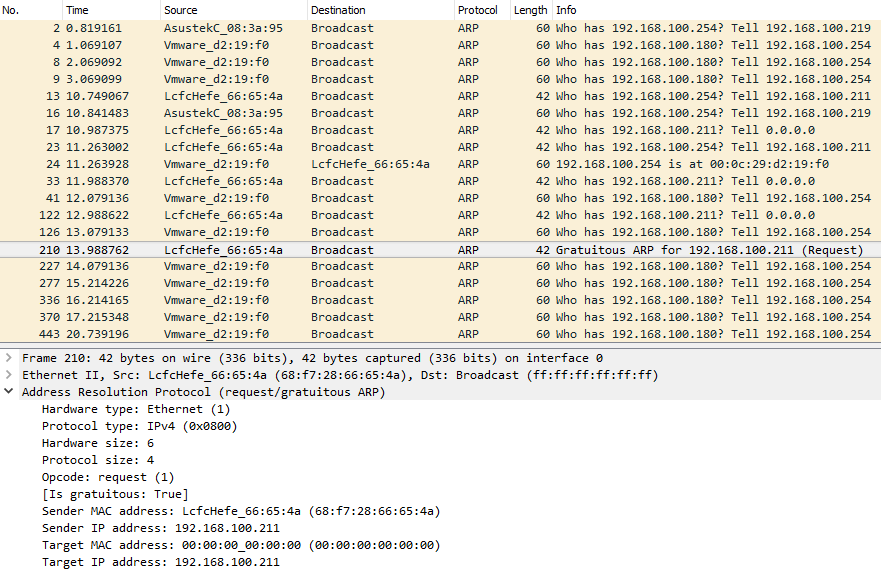
\includegraphics[width=0.98\linewidth]{./imagens/ARPG2_1.png}
  \end{subfigure}%
  \begin{subfigure}{.4\textwidth}
    \centering
    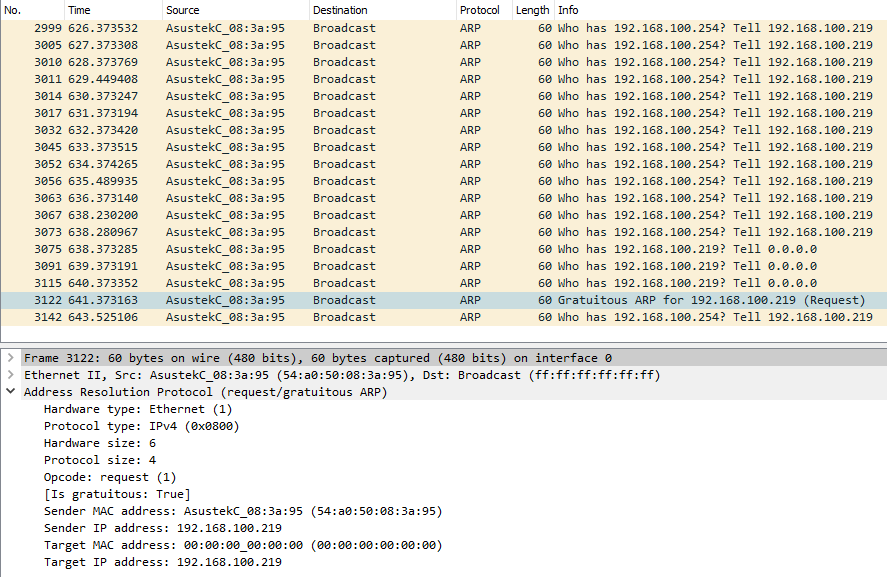
\includegraphics[width=0.98\linewidth]{./imagens/ARPG2_2.png}
  \end{subfigure}%
  \caption{2 pacotes de ARP Gratuito capturados com um intervalo de 627s.}
  \label{fig:arpg_2}
\end{figure}


\clearpage
\subsection{Exercício 2}
\subsubsection{Questão}\rule[-10pt]{0pt}{10pt}\\

Analise o conteúdo de um pedido ARP gratuito e identifique em que se distingue dos restantes pedidos ARP. Registe a trama Ethernet correspondente. Qual o resultado esperado face ao pedido ARP gratuito enviado?

\subsubsection{Resposta}\rule[-10pt]{0pt}{10pt}\\

O pacote de pedido ARP Gratuito difere dos restantes em que o IP de envio é igual ao IP destino. Como o destino da trama Ethernet é ff:ff:ff:ff:ff:ff (endereço de broadcast), este irá enviar o pacote a todos os hosts da rede. Estes, por sua vez, ao receber o pacote - e identificando o pacote como ARP Gratuito - irão atualizar as respetivas tabelas ARP no MAC em questão com o novo IP.

\subsubsection{Realização}\rule[-10pt]{0pt}{10pt}\\

\begin{figure}
  \begin{center}
    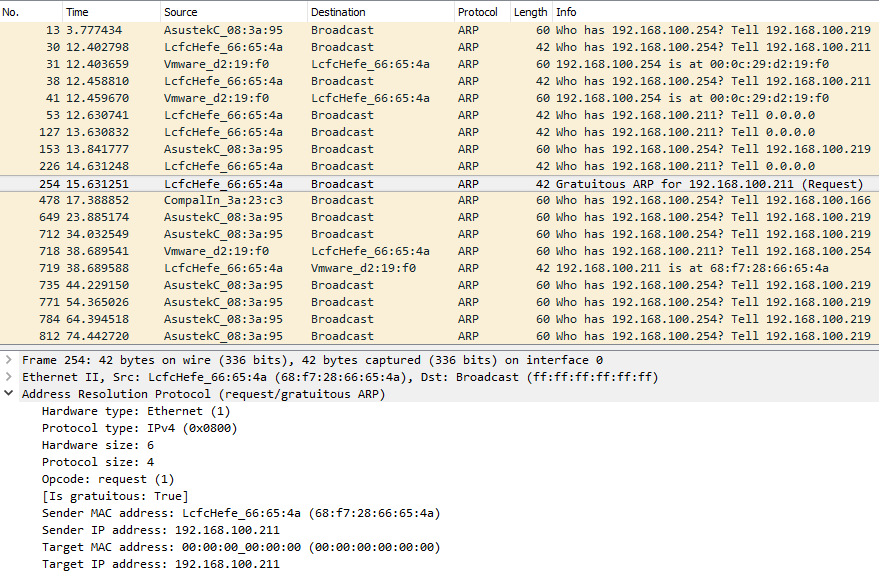
\includegraphics[scale=0.6]{./imagens/ARPG_IP.png} 
  \end{center}
  \caption{O IP destino é igual ao IP fonte e o destino Ethernet é \textit{Broadcast}.}
  \label{fig:arpg_ip}
\end{figure} 


\clearpage
\section{Parte II - Domínios de colisão}

\subsection{Exercício 1}
\subsubsection{Questão}\rule[-10pt]{0pt}{10pt}\\

Faça ping de n1 para n4. Verifique com a opção tcpdump como flui o tráfego nas diversas interfaces dos vários dispositivos. Que conclui?

\subsubsection{Resposta}\rule[-10pt]{0pt}{10pt}\\

A rede criada no CORE encontra-se ligada por um \textbf{repetidor}, que quando recebe tramas de um determinado \textit{host} apenas reproduz essa informação para todas as redes a qual se encontram ligadas e como tal pode existir colisões entre diferentes tramas. Deste modo, quando é feito \emph{ping de n1 para n4} todos os restantes \textit{hosts} ficam à espera que as ligações fiquem livres para poderem voltar a enviar tramas. Efetivamente, ficam à escuta do que vai passando na rede. Consequentemente o \textit{tcpdump} apresenta os pacotes que estão a ser enviados do n1 para o n4, além de que mais nenhuma trama circula na rede a não ser as trocadas entre o n1 e o n2.

Concluindo, os resultados apresentados verificam o modo como as colisões são evitadas, ou seja, é utilizado o protocolo CSMA/CD para resolver as colisões neste domínio de colisão em específico \cite{wiki:csma}.

\subsubsection{Realização}\rule[-10pt]{0pt}{10pt}\\

\begin{figure}
  \begin{center}
	  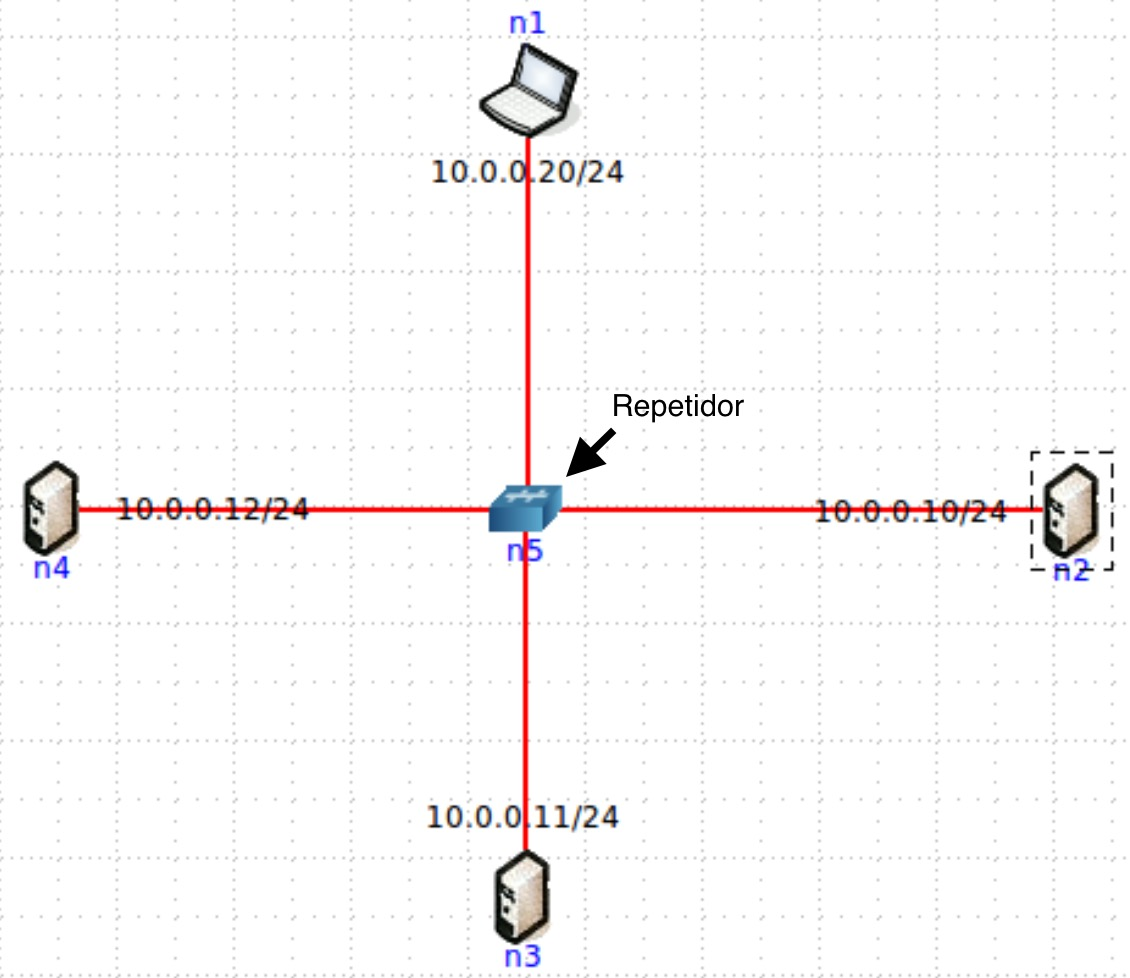
\includegraphics[scale=0.2]{./imagens/rede_23_repetidor.png} 
  \end{center}
	\caption{Topologia de rede que utiliza um repetidor.}
  \label{fig:rede_23_repetidor}
\end{figure} 

\begin{figure}
  \begin{center}
	  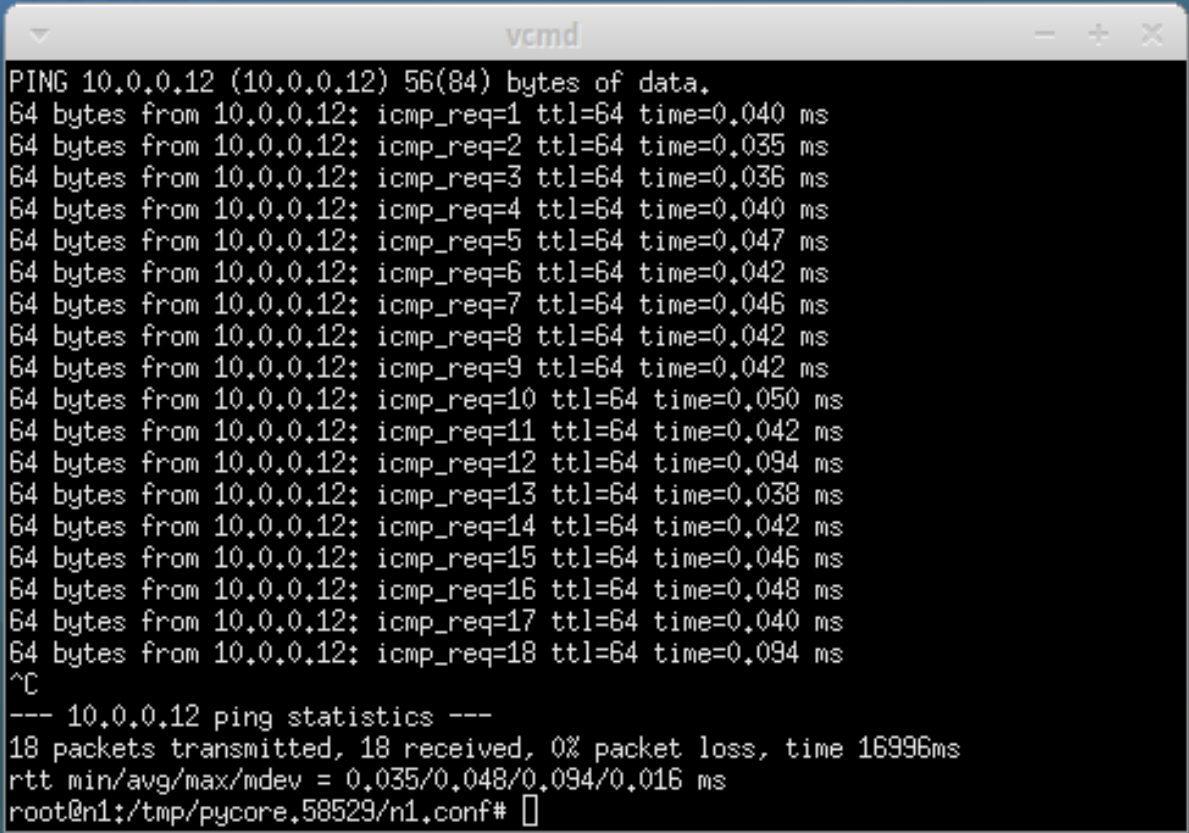
\includegraphics[scale=0.3]{./imagens/n1_repetidor.png} 
  \end{center}
	\caption{\texttt{Ping} realizado do \textit{host} n1 para o \textit{host} n4.}
  \label{fig:n1_repetidor}
\end{figure} 

\begin{figure}
  \begin{center}
	  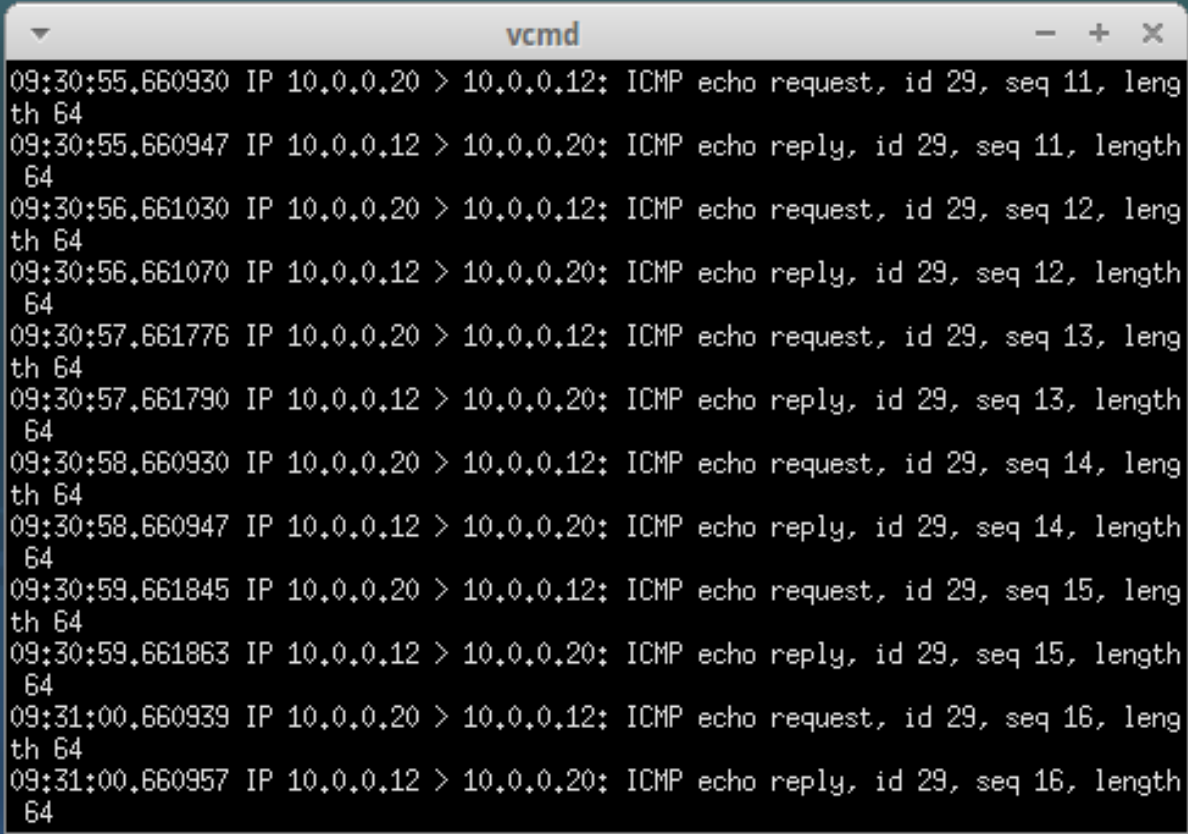
\includegraphics[scale=0.3]{./imagens/n2_tcpdump_repetidor.png} 
  \end{center}
	\caption{\texttt{Tcpdump} no \textit{host} n2.}
  \label{fig:n2_repetidor}
\end{figure} 

\begin{figure}
  \begin{center}
	  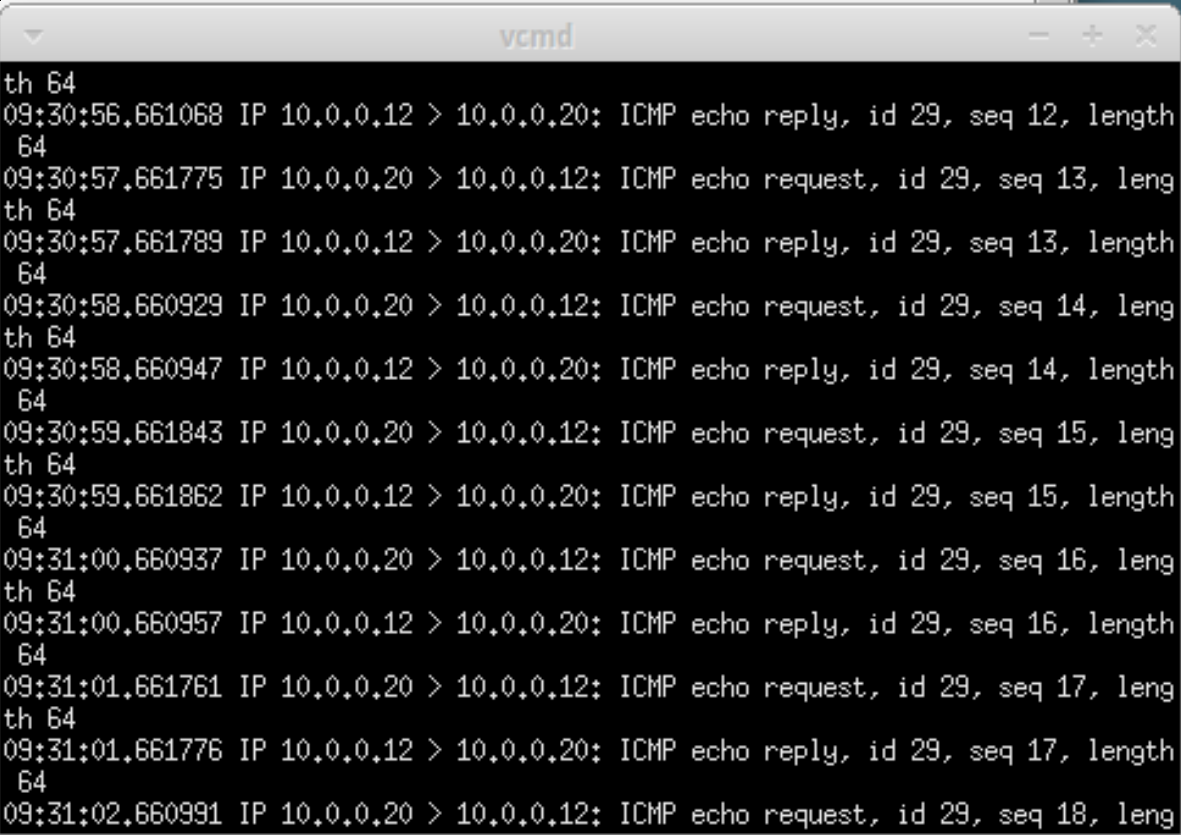
\includegraphics[scale=0.3]{./imagens/n3_tcpdump_repetidor.png} 
  \end{center}
	\caption{\texttt{Tcpdump} no \textit{host} n3.}
  \label{fig:n3_repetidor}
\end{figure} 

\begin{figure}
  \begin{center}
	  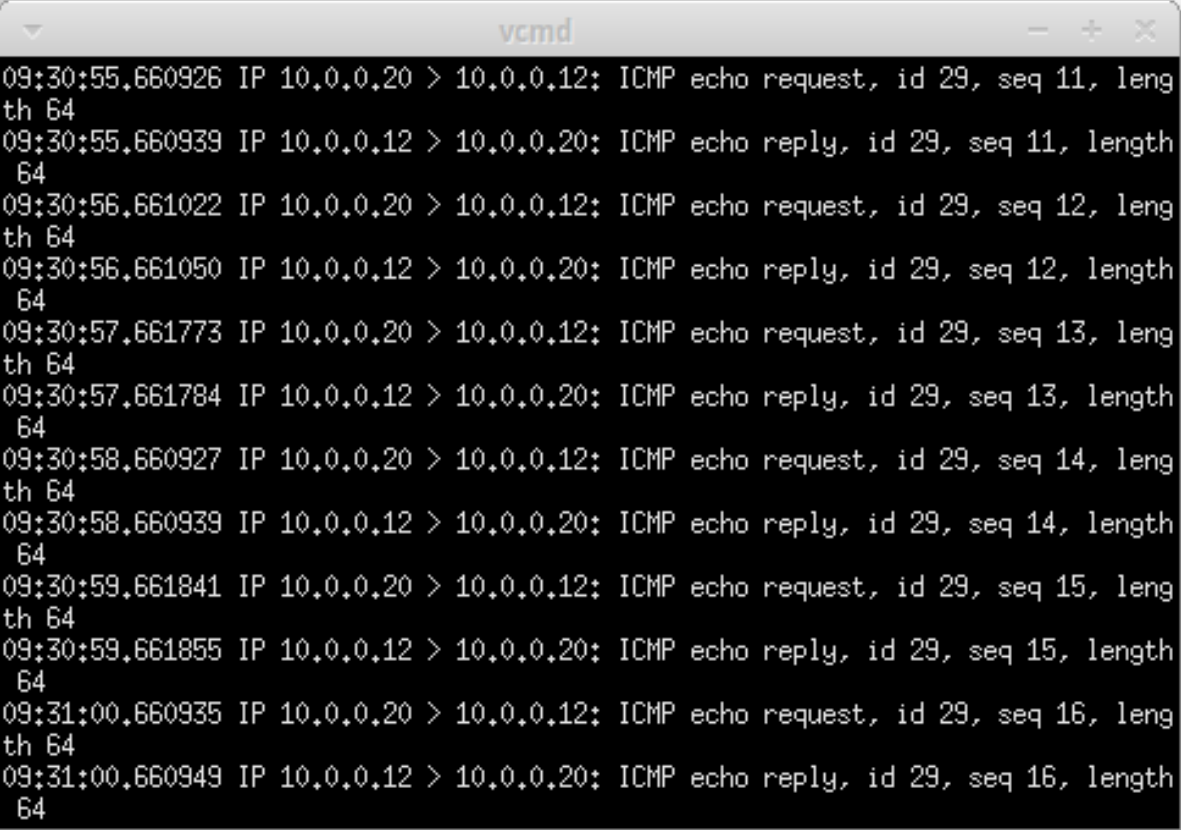
\includegraphics[scale=0.3]{./imagens/n4_tcpdump_repetidor.png} 
  \end{center}
	\caption{\texttt{Tcpdump} no \textit{host} n4.}
  \label{fig:n4_repetidor}
\end{figure} 

\clearpage
\subsection{Exercício 2}
\subsubsection{Questão}\rule[-10pt]{0pt}{10pt}\\

Na topologia de rede substitua o hub por um switch. Repita os procedimentos que realizou na pergunta anterior. Comente os resultados obtidos quanto à utilização de hubs e switches no contexto de controlar ou dividir domínios de colisão. Documente as suas observações e conclusões com base no tráfego observado/capturado.

\subsubsection{Resposta}\rule[-10pt]{0pt}{10pt}\\

Substituindo o repetidor pelo \textit{switch} as colisões são evitadas. Essa diferença é resultado da metodologia na qual o \textit{switch} acenta. Efetivamente, este aprende a rede na qual se encontra inserido e constrói uma tabela com os endereços MAC correspondendo-os às respetivas portas a que os sistemas se encontram ligados. Assim quando o \textit{host} n1 realiza \textit{ping} no \textit{host} n4, o \textit{switch} reencaminha o tráfego diretamente na porta na qual o n4 está ligado. Desta forma colisões entre diferentes segmentos deixam de ser possíveis visto estarem efetivamento separados. Como resultado, o \textit{tcpdump} que se encontra a correr no \textit{host} n2 e n3, não apresenta qualquer tráfego resultante do \textit{ping} entre o \textit{host} n1 e n4, pois o tráfego encontra-se isolado destes sistemas \cite{wiki:comutador}.

\subsubsection{Realização}\rule[-10pt]{0pt}{10pt}\\

\begin{figure}
  \begin{center}
	  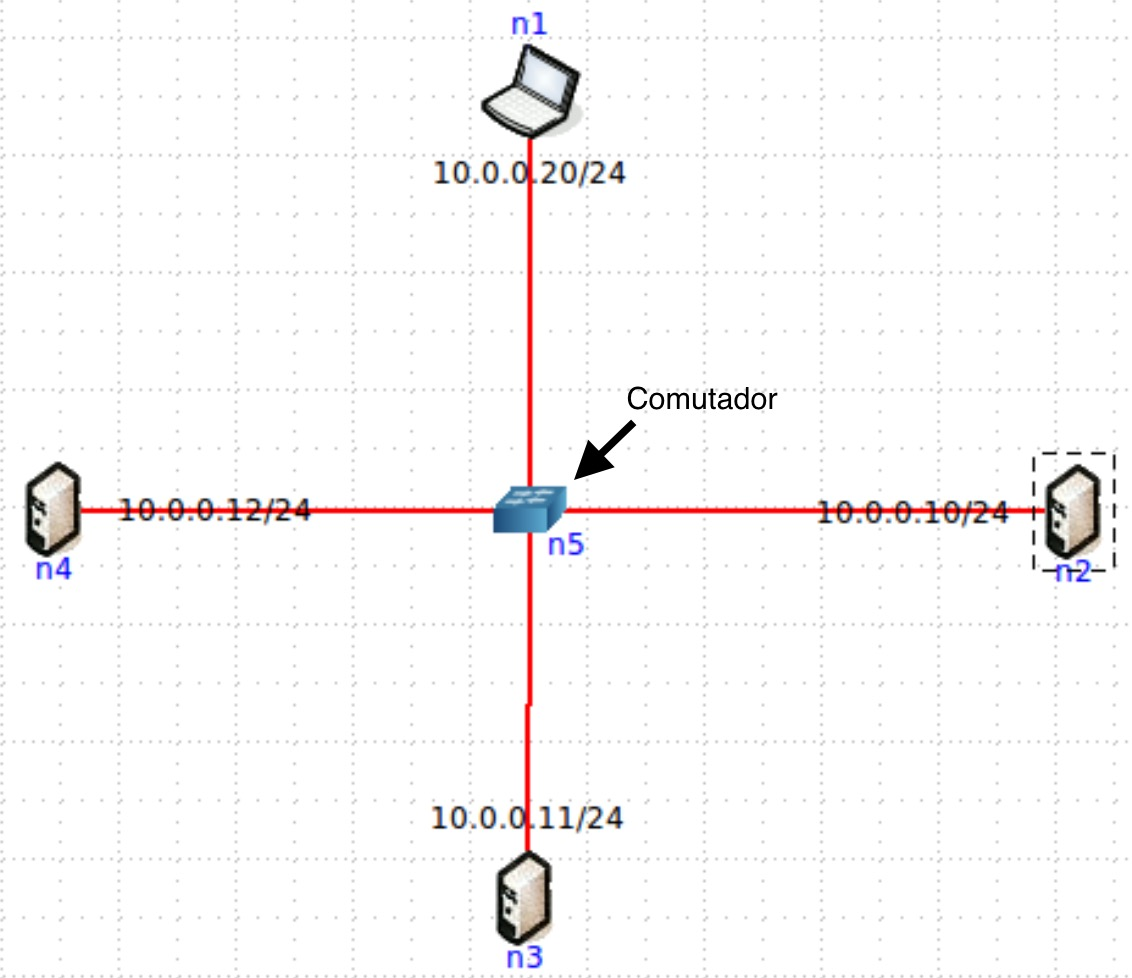
\includegraphics[scale=0.2]{./imagens/rede_23_comutador.png} 
  \end{center}
	\caption{Topologia de rede que utiliza um comutador.}
  \label{fig:rede_23_comutador}
\end{figure} 

\begin{figure}
  \begin{center}
	  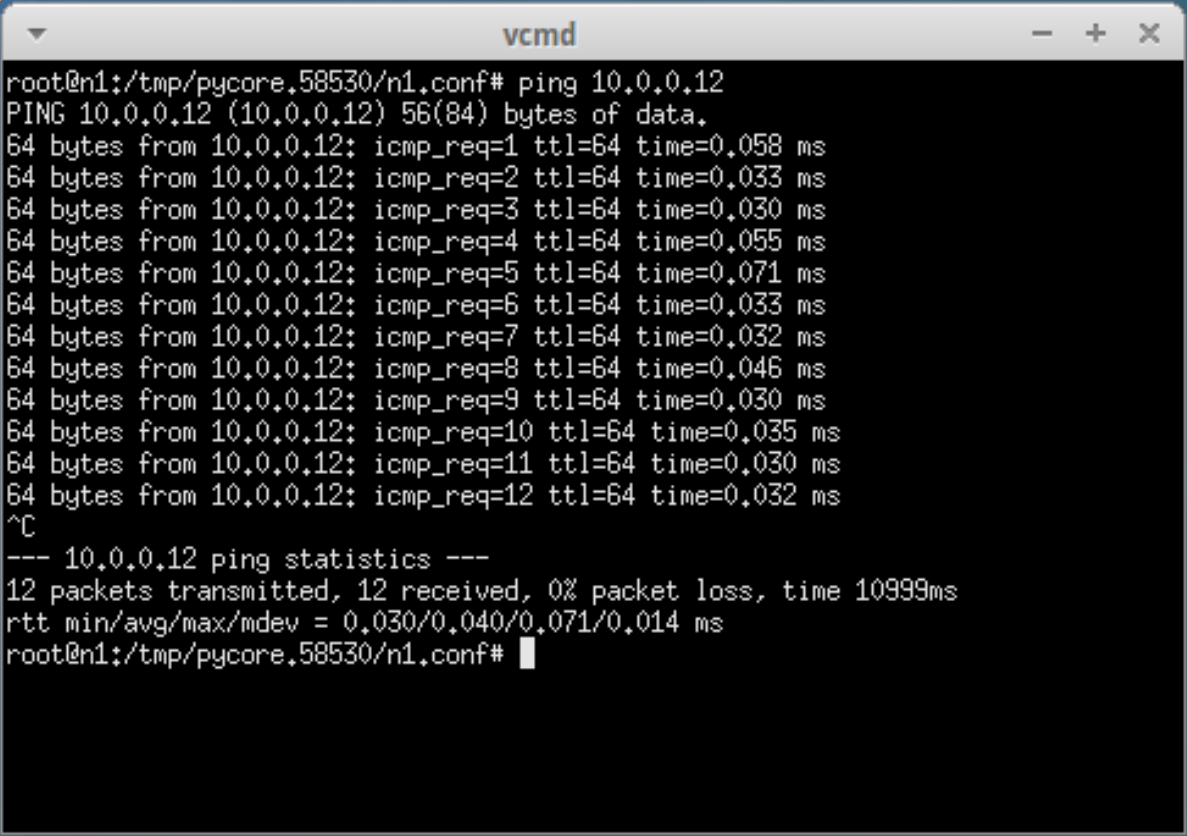
\includegraphics[scale=0.3]{./imagens/n1_comutador.png} 
  \end{center}
	\caption{\texttt{Ping} realizado do \textit{host} n1 para o \textit{host} n4.}
  \label{fig:n1_comutador}
\end{figure} 

\begin{figure}
  \begin{center}
	  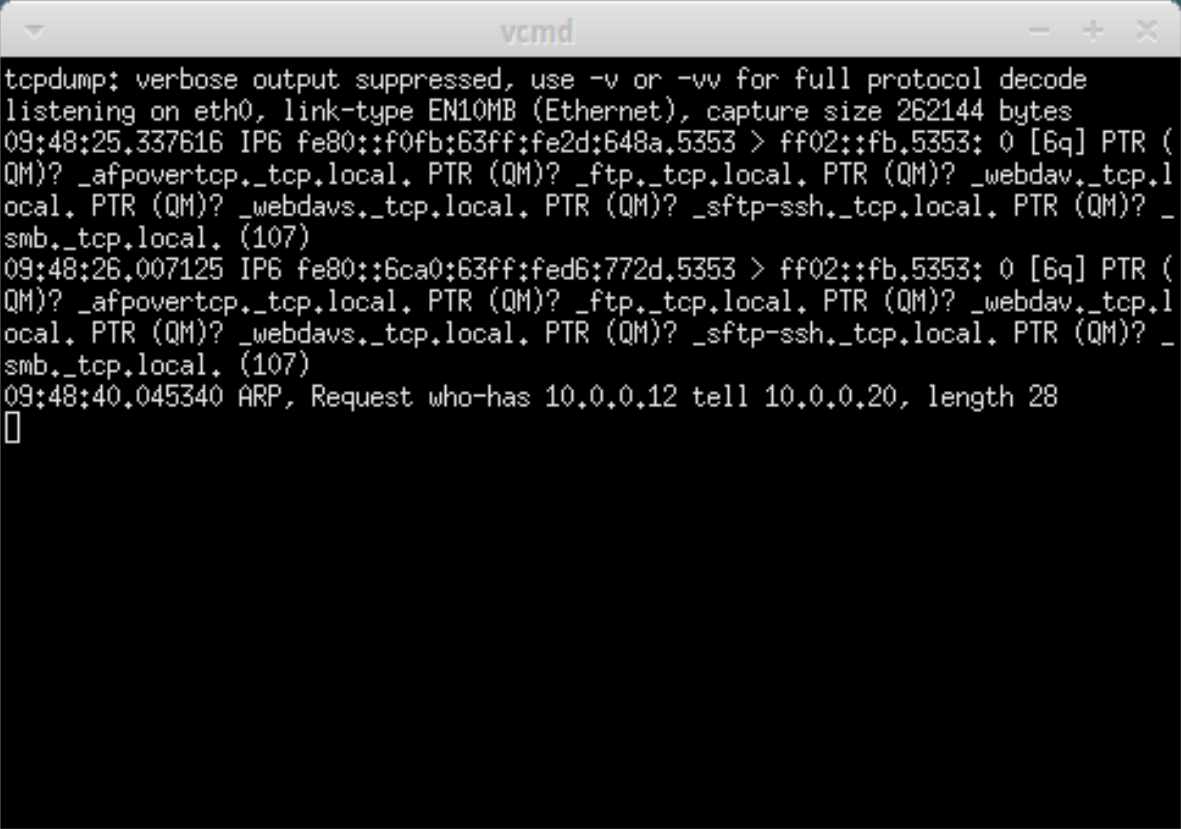
\includegraphics[scale=0.3]{./imagens/n2_tcpdump_comutador.png} 
  \end{center}
	\caption{\texttt{Tcpdump} no \textit{host} n2.}
  \label{fig:n2_comutador}
\end{figure} 

\begin{figure}
  \begin{center}
	  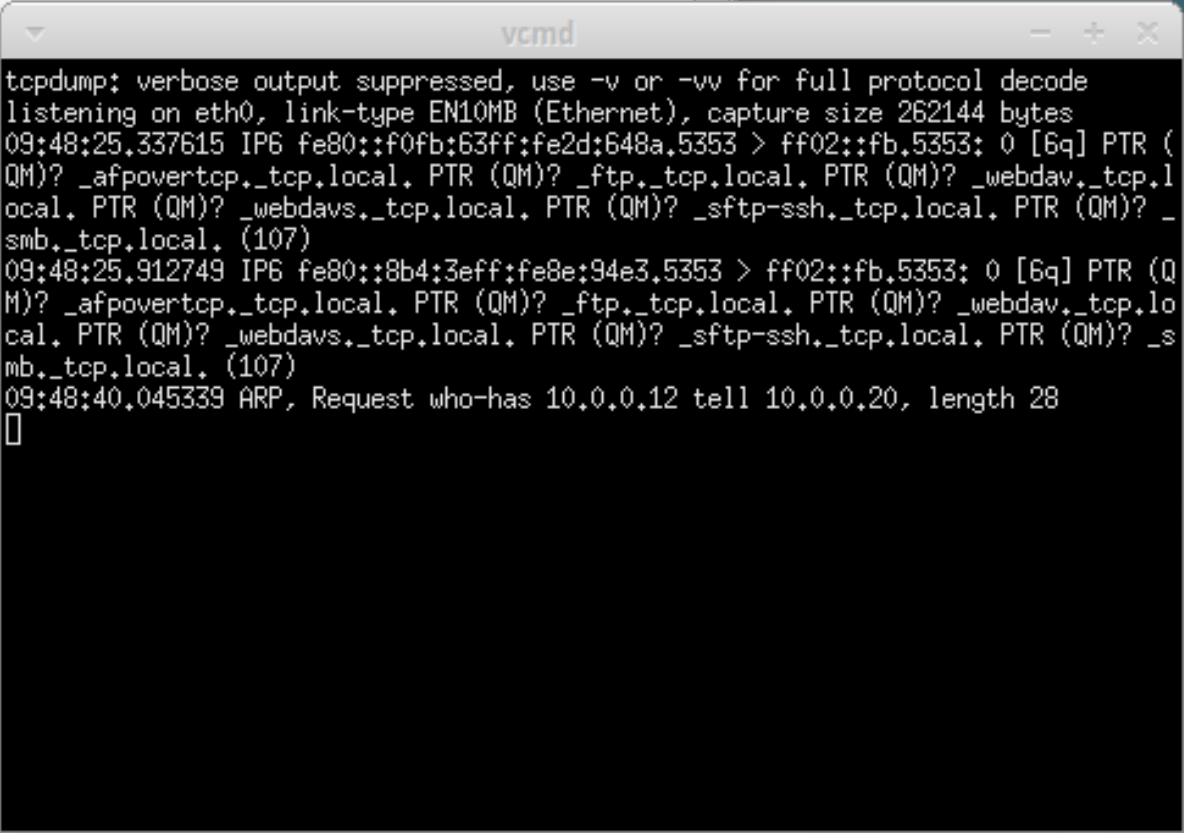
\includegraphics[scale=0.3]{./imagens/n3_tcpdump_comutador.png} 
  \end{center}
	\caption{\texttt{Tcpdump} no \textit{host} n3.}
  \label{fig:n3_comutador}
\end{figure} 

\begin{figure}
  \begin{center}
	  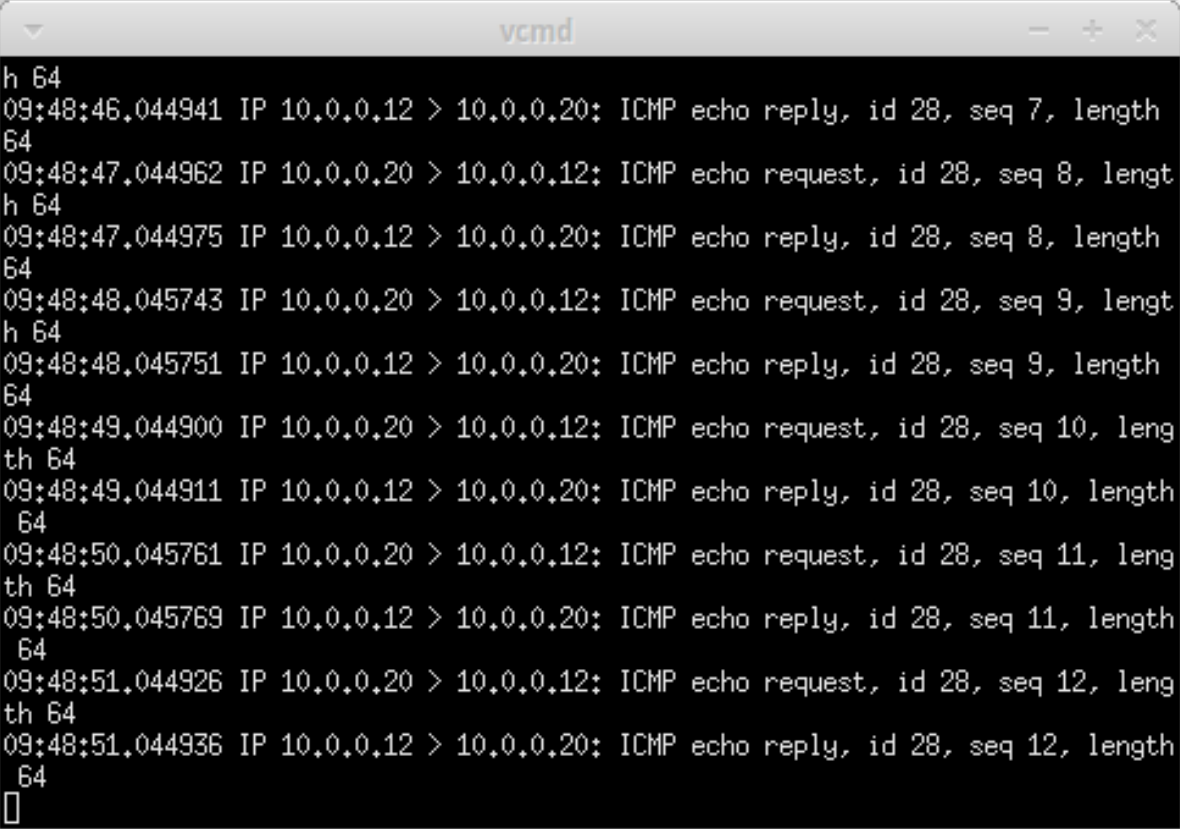
\includegraphics[scale=0.3]{./imagens/n4_tcpdump_comutador.png} 
  \end{center}
	\caption{\texttt{Tcpdump} no \textit{host} n4.}
  \label{fig:n4_comutador}
\end{figure} 

\clearpage

\section{Conclusões}
Neste trabalho...

%BIBLIOGRAFIA
\bibliographystyle{splncs}
\bibliography{ficheirodebibliografia}

\end{document}
